\documentclass{letter}

\usepackage[a4paper]{geometry}
\usepackage{graphicx}

\begin{document}

\begin{center}
    \large\textbf{FOSSEE}
\end{center}

\textbf{Free and Open Source Software in Education} (http://fossee.in) provides 
free support on FOSS (free and open source software) to eliminate the use of 
proprietary/commercial software packages in Science and Engineering Education 
across India. The shift to FOSS packages will help educational institutions 
monetarily. 

The flagship activities promoted by the FOSSEE team are:

\begin{enumerate}

\item \textbf{SELF Workshops} are Spoken Tutorial (ten minute audio-video 
tutorial suitable for self learning) based workshops. FOSSEE has created various 
FOSS Spoken Tutorials that are used for Self workshops conducted remotely from 
IIT Bombay.  Students and faculty across the country undertake these workshops 
where they learn different FOSS tools. FOSSEE offers domain expertise for these 
workshop(s) and also set online exams that are conducted at the end of the 
workshop. During the last one year, a total of 695 SELF workshops on various 
FOSS tools have been conducted, training about 22,000 students and faculty 
members. Post workshop(s), students post queries, if any, on \textbf{Spoken 
Tutorial Forum }(http://forums.spoken-tutorial.org/) for any of the existing 
FOSS series and are given quick answers from FOSSEE domain experts.

\vskip3ex

\item One of the major shortcomings of FOSS tools is the lack of documentation.  
FOSSEE addresses this important issue by promoting \textbf{Textbook Companion} 
activity by creating codes for solved examples of standard textbooks using FOSS.  
It is available online  for free download and use and the contributors are 
students and the faculty of colleges from different parts of India.

\vskip3ex

\item Lab Migration: As long as a college uses proprietary tools as part of 
their lab curriculum, we cannot eliminate the use of commercial software.  To 
address this issue, we have started the \textbf{Lab Migration} activity that 
aims to migrate college labs using proprietary software to a FOSS only lab.  The 
FOSS code created by a student/teacher is released in open source code for 
public use. \\

Students and faculty involved in Textbook Companion and Lab Migration are given 
honorarium for their efforts.

\vskip3ex

\item \textbf{Conference}: Scipy India - an international conference on 
scientific computing with Python, is organized every year by FOSSEE since 2009.  
One of the goals of the conference is to combine education, engineering, and 
science with computing through the medium of Python.

\end{enumerate}

\newpage
Currently, FOSSEE team promotes the following software extensively: \\

% first column
\begin{minipage}[t]{0.5\linewidth}
    \begin{center}
        
\includegraphics[width=0.8\linewidth]{images/scilab_logo.png}
    \end{center}
\textbf{Scilab} is a free and open source software for numerical computation 
developed by Scilab Enterprises, France. It is a FOSS alternative to MATLAB.  It 
also includes Xcos which is an open source alternative to Simulink. The Scilab 
team have successfully created more than 275 Textbook Companions and ported 12 
labs through the Lab Migration activity till date. To increase ease of executing 
Textbook Companion code online, FOSSEE has ported TBC on GARUDA cloud 
(http://scilab.in/scilab-on-cloud). Please visit http://scilab.in for more 
details.
\end{minipage} \hspace{1cm}
%second column
\begin{minipage}[t]{0.5\linewidth}
    \begin{center}
        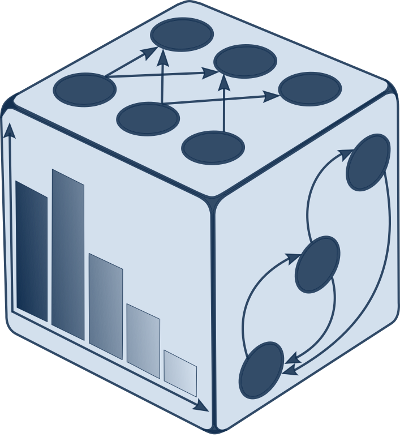
\includegraphics[width=0.3\linewidth]{images/coin_logo.png}
    \end{center}
\textbf{COIN-OR} or \textbf{CO}mputational \textbf{IN}frastructure for 
\textbf{O}perations \textbf{R}esearch is a project to build and support an 
open-source software for operations research and its applications.  
\textbf{Simpy} (Simulation in Python) is an open source, Python-based, 
discrete-event simulation software. OR Tools at FOSSEE is promoting COIN-OR, 
Simpy and other FOSS by developing tutorials, textbook companions and software 
interfaces in Scilab and Python. For more details please visit 
http://or.fossee.in
\end{minipage}

% first column
\begin{minipage}[t]{0.5\linewidth}
    \begin{center}
        
\includegraphics[width=0.37\linewidth]{images/cfd_logo.png}
    \end{center}
\textbf{OpenFOAM} is a free, open source CFD software package developed by 
OpenCFD Ltd and distributed by the OpenFOAM Foundation. Tutorials in the form of 
web-casts, for self learning OpenFOAM have been developed by our team. These are 
available free of cost at http://cfd.fossee.in.
\end{minipage} \hspace{1cm}
%second column
\begin{minipage}[t]{0.5\linewidth}
    \begin{center}
        
\includegraphics[width=0.35\linewidth]{images/python_logo.png}
    \end{center}
\textbf{Python} is a general-purpose interpreted, high-level, object-oriented 
programming language that is used in a wide variety of application domains.The 
Python team promotes the use of the language through Python Textbook Companion.  
Under Python Textbook Companion, 53 textbook companions have been completed. For 
more information visit http://python.fossee.in/
\end{minipage}

\begin{minipage}[t]{0.5\linewidth}
    \begin{center}
        
\includegraphics[width=0.35\linewidth]{images/oscad_logo.png}
    \end{center}
\textbf{Oscad} is developed by the FOSSEE team at IIT Bombay it is an EDA tool 
for circuit design, simulation, analysis and PCB design. Free tutorials of Oscad 
are available at http://oscad.in/resources/tutorials.
\end{minipage}

\end{document}
